\section{Introduction}
\label{sec:introduction}

  % Nécessité de l'analyse temporelle pour le temps-reél.

  L'analyse temporelle d'une tâche vise à déterminer une borne supérieure sur
  son temps d'exécution pour un matériel spécifique. Il est nécessaire d'estimer
  de manière sûre et précise ces bornes afin de pouvoir déterminer des
  ordonnancements et réaliser des analyses de faisabilité garantissant le
  respect de l'ensemble des contraintes temporelles des systèmes temps-réel.

  % Nécessité de la reconstruction de CFG pour l'analyse temporelle.

  Le temps d'exécution d'une tâche dépend de son chemin d'exécution et du temps
  d'exécution de chaque instruction de ce chemin. Afin de procéder à l'analyse
  temporelle d'une tâche, il est donc nécessaire d'en obtenir le graphe de flot
  de contrôle (\textit{Control Flow Graph} ou CFG). En effet, le CFG d'une tâche
  représente tous les chemins qu'elle peut suivre à l'exécution. Il est
  cependant très rare que le CFG d'une tâche soit disponible. Il est alors
  nécessaire de procéder à une reconstruction de celui-ci.

  \vspace{1em}
  
  % Intérêt de la vérification de modèle pour l'analyse temporelle.

  \begin{figure}[ht]
    \centering
    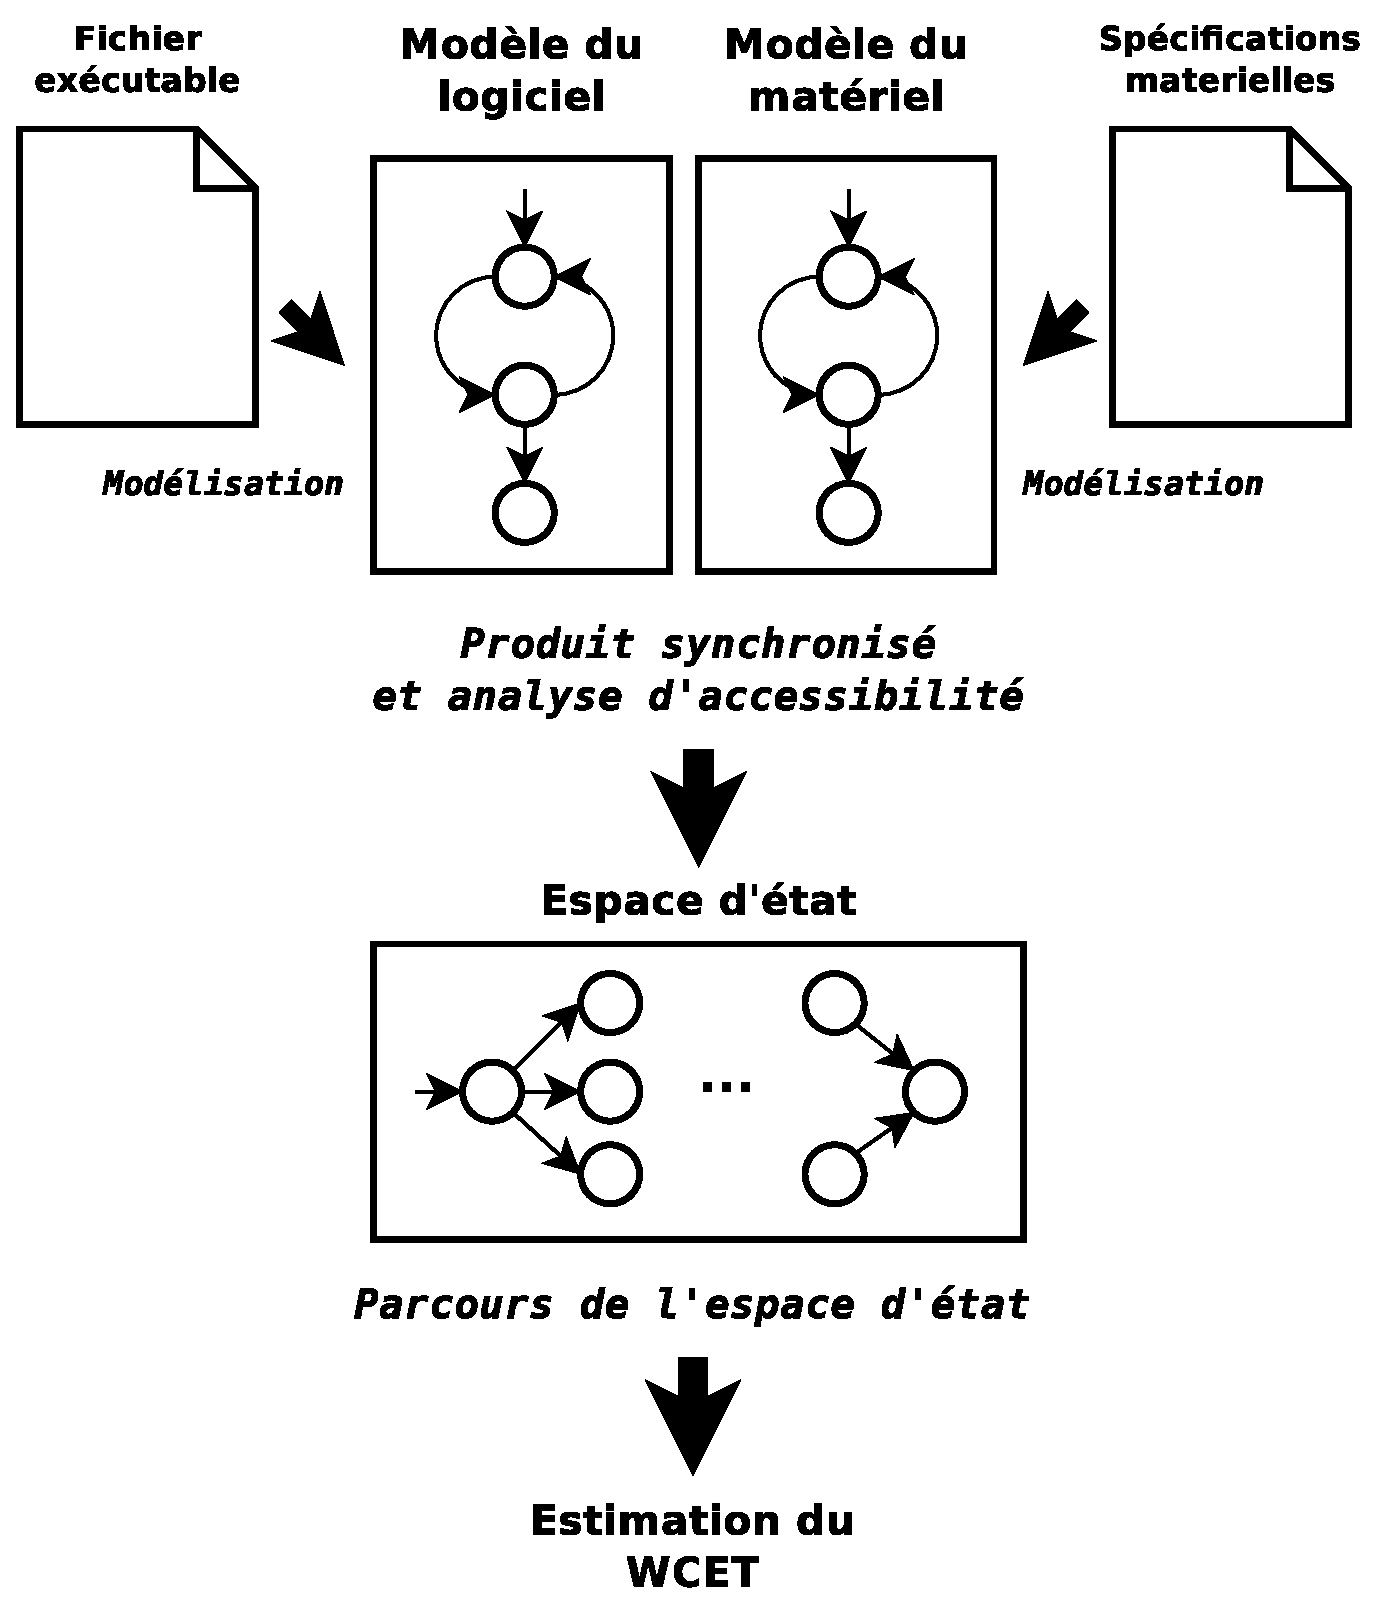
\includegraphics[scale=0.3]{img/model-checking.eps}
    \caption{Principes de l'analyse temporelle par vérification de modèles}
    \label{fig:model-checking}
  \end{figure}

  Différentes approches d'analyse temporelle se basent sur la vérification de
  modèles temporisés. Elles consistent en la vérification du produit synchronisé
  du modèle du programme et du modèle de la plateforme materielle -- cf. figure
  \ref{fig:model-checking}. L'analyse temporelle est alors réduit à un problème
  d'accessibilité temporisée. Ce problème est solvable grâce aux méthodes de
  vérification de modèles temporisés existantes.

  Il existe différents outils d'analyse temporelle à base de vérification de
  modèle \cite{DOT10, CB13}. Les résultats expérimentaux montrent qu'une prise
  en compte moins abstraite des comportements matériels produit des estimations
  du pire cas de temps d'exécution plus précises. Cependant, ces outils
  n'offrent pas de performances acceptables du fait d'une trop forte expansion
  de leur espaces d'état \cite{Wil04}.

  \vspace{1em}

  % Utilisation d'une bibliothèque d'analyse et de transformation de CFG pour le
  % slicing de CFG.
  % Organisation de l'article.

  L'outil d'analyse statique de fichier binaire détaillé ici est implémenté en
  Haskell grace à Hoopl, une bibliothèque de manipulation de CFG
  \cite{RDP10}. Cette bibliothèque permet de définir simplement des analyses de
  flots de données ainsi que des transformations sur les CFG manipulés. La
  section \ref{sec:reconstruction} détaille le processus de reconstruction de
  CFG et la section \ref{sec:simplification} détaille le processus de
  \textit{simplification} de CFG. La section \ref{sec:related-work} évoque
  différentes méthodes de reconstruction de CFG existantes. Enfin, la section
  \ref{sec:conclusion} présente les perspectives de ce travail.
